% Self-contained manuscript; generated by paper/assemble.py.
\documentclass[11pt,letterpaper]{article}
\usepackage[T1]{fontenc}
\usepackage{lmodern}
\usepackage[margin=1in]{geometry}
\usepackage{amsmath,amssymb,booktabs,tabularx,array,microtype}
\usepackage{caption,placeins,graphicx}

% BEGIN figures/plots/style.tex
\usepackage{tikz,pgfplots}
\usetikzlibrary{arrows.meta,positioning,calc}
\pgfplotsset{compat=1.18,every axis/.append style={font=\fontsize{10}{12}\selectfont,axis line style={line width=.4pt},tick style={line width=.4pt},major tick length=2pt,axis lines*=left,scaled ticks=false,grid=none,legend style={draw=none,fill=none,font=\fontsize{10}{12}\selectfont},label style={font=\fontsize{10}{12}\selectfont},title style={font=\fontsize{10}{12}\selectfont},tick label style={font=\fontsize{10}{12}\selectfont}}}
\tikzset{flow/.style={-{Latex[length=1.6mm]},line width=.5pt},stage/.style={draw,line width=.5pt,minimum height=7mm,align=center,inner sep=3pt,font=\fontsize{10}{12}\selectfont}}

% END figures/plots/style.tex

\usepackage{helvet}

% BEGIN figures/schematics/style.tex
\usepackage[T1]{fontenc}
\usepackage{lmodern,helvet,amsmath,amssymb,tikz}
\usetikzlibrary{arrows.meta,calc,positioning}
\definecolor{accent}{HTML}{315C7C}
\definecolor{tint}{HTML}{EAF0F5}
\definecolor{rule}{HTML}{B7BEC4}
% END figures/schematics/style.tex

\usepackage[hidelinks]{hyperref}
\captionsetup{font=small,labelfont=bf}
\setlength{\parskip}{2pt}
\setlength{\emergencystretch}{1.5em}
\widowpenalty=10000
\clubpenalty=10000
\displaywidowpenalty=10000
\pagestyle{plain}
\newcommand{\model}{ModalStripe}
\newcommand{\R}{\mathbb{R}}
\title{ModalStripe: Modal Memory and Attention\\in Small Language Models}
\author{Atay Kim\\[3pt]\normalsize Nazarbayev University\\\normalsize Astana, Kazakhstan\\\normalsize\href{mailto:atay.kim@nu.edu.kz}{\texttt{atay.kim@nu.edu.kz}}}
\date{\small November 5, 2026\quad (v0.5)}
\hypersetup{pdftitle={ModalStripe: Modal Memory and Attention in Small Language Models},pdfauthor={Atay Kim},pdfsubject={Version 0.5, November 5, 2026}}
\begin{document}
\maketitle
\begin{abstract}
We study whether a small language model benefits from combining modal memory with attention. ModalStripe replaces one of two global-attention blocks with a gated modal convolution followed by local attention. On two books excluded from training and primary model selection, it reaches character perplexity 5.592, compared with 6.047 for full attention and 5.964 for a local-plus-global control at the same training-character budget. The result persists with fixed feed-forward widths, but the advantage over attention falls to about 1.9\% under a timing-calibrated training budget. CPU latency improves at long prefixes and the retained cache is roughly halved; most of that cache saving also occurs without the modal branch. A local-only baseline is a strong resource alternative, and prediction quality deteriorates beyond the trained context. The modal branch improves prediction at this scale; its training cost reduces the advantage under timing calibration.
\end{abstract}

\section{Introduction}
A hybrid language model can use less global attention without becoming a better model in practice. It may need more training, save cache while adding latency, or run quickly at a context length where its predictions have become worse. A useful comparison has to measure these effects together.

This paper examines one such design. \model\ has two blocks: the first combines a gated modal convolution with local attention, and the second retains full causal attention. The modal branch uses damped complex exponentials, allowing the same operator to run as an FFT convolution on complete sequences and as a compact recurrence during decoding. We compare it with two global-attention blocks and with a local-plus-global model that removes only the modal branch.

The experiments are deliberately small: width-64 character models, three optimization seeds, and transfer to two books. That scale makes a controlled audit practical, but limits what the results can establish. The main question is whether the modal branch earns its cost under explicit data, parameter and timing budgets. We find a consistent gain at equal training characters, a smaller gain after timing calibration, and meaningful weaknesses in context extrapolation. We also retain unfavorable results and distinguish the original comparisons from later exploratory checks.

\section{Relation to existing models}
ModalStripe uses established sequence-modeling ideas. Structured state-space models such as S4 provide recurrent and convolutional views of long-sequence operators \cite{s4}. H3 studies recall limitations and attention hybrids \cite{h3}; Hyena combines long convolutions with data-controlled gates \cite{hyena}; and StripedHyena~2 develops convolutional multi-hybrids at scale \cite{stripedhyena}. These models provide the starting point for our study. We compare small, controlled implementations to understand what the modal branch contributes.

The connection to Fourier neural operators \cite{fno} is spectral computation, not demonstrated PDE-learning or resolution-transfer behavior. Zoology motivates separating language prediction from associative recall \cite{zoology}; state-space duality and gated delta networks offer further approaches to efficient interaction and memory updates \cite{ssd,deltanet}. Our character-perplexity results do not measure their capabilities or establish a new hybrid-model family.

\section{Model and comparisons}
All models start from random weights and share a fixed 128-symbol ASCII inventory, two blocks, width 64, four attention heads, sinusoidal positions \cite{vaswani}, and an untied prediction head. A common causal stem adds a linear projection of the previous character embedding. Each mixer has a normalized residual update, followed by a normalized, two-layer GELU feed-forward network. There is no dropout.

The full-attention baseline uses global causal attention in both blocks. The local-plus-global control uses a window-8 local block followed by a global block. \model\ inserts the modal mixer before local attention in the first block. Both mixers act sequentially, sharing the block's first layer-normalization parameters. The global block is retained. Appendix~\ref{app:methods} gives the full block definition and initialization.

\begin{figure}[htbp]
\centering\resizebox{\textwidth}{!}{
\begingroup
\tikzset{every node/.style={font=\sffamily\fontsize{9.5}{11.5}\selectfont},
module/.style={draw=black!75,line width=.55pt,fill=white,minimum height=.78cm,align=center,inner xsep=6pt,inner ysep=5pt},
focal/.style={module,fill=tint,draw=accent,line width=.7pt},
flow/.style={-{Latex[length=1.6mm,width=1.1mm]},line width=.6pt,draw=black!85},
label/.style={font=\sffamily\fontsize{9.5}{11.5}\selectfont,align=center},
heading/.style={font=\sffamily\bfseries\fontsize{10}{12}\selectfont,anchor=west},
op/.style={draw=black!80,circle,fill=white,inner sep=0pt,minimum size=4.8mm,font=\normalsize}}
\hyphenpenalty=10000
\exhyphenpenalty=10000

% BEGIN figures/schematics/01-intervention.tex
\begin{tikzpicture}[x=1cm,y=1cm]
\node[heading] at (0,8.55) {(a) Two-block language model};
\node (tokens) at (.25,7.5) {$x_{0:T-1}$};
\node[module,text width=1.65cm] (stem) at (2.5,7.5) {Input stem};
\node[focal,text width=2.65cm] (b1) at (6.1,7.5) {First block $B_1$};
\node[module,text width=3.2cm] (b2) at (10.65,7.5) {Global-attention\\block $B_2$};
\node[module,text width=1.85cm] (head) at (14.9,7.5) {Output head};
\node (logits) at (17.1,7.5) {$\ell_{0:T-1}$};
\foreach \a/\b in {tokens/stem,stem/b1,b1/b2,b2/head,head/logits}{\draw[flow] (\a.east)--(\b.west);}

\draw[rule,line width=.45pt] (0,6.15)--(17.65,6.15);
\node[heading] at (0,5.7) {(b) First-block alternatives};
\foreach \id/\x/\name in {g/2.8/Full attention,l/8.55/Local + global,m/14.3/ModalStripe}{
\node[font=\sffamily\fontsize{10}{12}\selectfont] at (\x,5.0) {\name};
\node (in\id) at (\x,4.42) {$H^{(0)}$};
\node[module,text width=3.65cm] (ff\id) at (\x,.95) {Feed-forward\\$\mathcal R_F$};
\node (out\id) at (\x,.05) {$H^{(1)}$};
\draw[flow] (ff\id.south)--(out\id.north);
}
\node[module,text width=3.65cm] (ag) at (2.8,3.5) {Global attention\\$\mathcal R_G$};
\node[module,text width=3.65cm] (al) at (8.55,3.5) {Local attention ($w=8$)\\$\mathcal R_L$};
\node[focal,text width=3.65cm] (modal) at (14.3,3.5) {Modal mixer\\$\mathcal R_M$};
\node[module,text width=3.65cm] (ml) at (14.3,2.22) {Local attention ($w=8$)\\$\mathcal R_L$};
\draw[flow] (ing.south)--(ag.north);
\draw[flow] (ag.south)--(ffg.north);
\draw[flow] (inl.south)--(al.north);
\draw[flow] (al.south)--(ffl.north);
\draw[flow] (inm.south)--(modal.north);
\draw[flow] (modal.south)--(ml.north);
\draw[flow] (ml.south)--(ffm.north);
\draw[rule,line width=.45pt] (0,-.55)--(17.65,-.55);
\node[label,anchor=north west,text width=17.3cm,align=left] at (0,-.8) {Every box in (b) is a pre-normalized residual update: $\mathcal R_f(H)=H+f(\operatorname{LN}(H))$. ModalStripe's modal and local updates reuse the same LayerNorm parameters. Feed-forward hidden widths depend on the allocation rule.};
\end{tikzpicture}

\endgroup
% END figures/schematics/01-intervention.tex
}
\caption{Model backbone and first-block alternatives. Each lower-panel box denotes a pre-normalized residual update. ModalStripe adds a modal update before local attention. All primary models retain the second global-attention block; weights are trained separately. Figure~\ref{fig:statecell} expands the modal decoding operator.}
\label{fig:architecture}
\end{figure}

For normalized input $a_t$, the modal branch writes
$u_t=(W_v a_t)\odot\sigma(W_w a_t)$ and reads through
$g_t=\sigma(W_r a_t)$. Its output is $W_o(z_t\odot g_t)$, where
\begin{equation}
 z_t=\sum_{j=0}^{t}K_{t-j}\odot u_j,\qquad
 K_{\ell,k}=\operatorname{Re}\sum_{r=1}^{8}c_{r,k}p_r^\ell,
 \quad p_r=e^{-\alpha_r+\mathrm{i}\omega_r},\quad\alpha_r>0.
 \label{eq:modal}
\end{equation}
Poles are shared across channels; complex residues are channel-specific. The kernel uses nonnegative lags, so zero-padding to at least $2T-1$ before FFT evaluation prevents circular wraparound. The equivalent decoding state is
\begin{equation}
 s_{t,r,k}=p_r s_{t-1,r,k}+u_{t,k},\qquad
 z_{t,k}=\operatorname{Re}\sum_r c_{r,k}s_{t,r,k}.
 \label{eq:state}
\end{equation}
This finite state belongs to the modal branch. The complete model still has a growing global KV cache and quadratic full-sequence attention work.

We test two allocation rules. Approximate parameter matching gives about 121,000 parameters per model, but reduces the mixed block's feed-forward width from 261 to 124. A second condition fixes every feed-forward width at 256, allowing the hybrid to have more parameters. Parameter matching is tested at both training contexts; fixed width is tested at context 128. The comparisons separate a similar total budget from a fixed feed-forward allocation.

\section{Experimental setup}
\paragraph{Data and training.}
Training uses the first 80\% of normalized \emph{Hamlet}, \emph{Alice's Adventures in Wonderland}, and \emph{Moby-Dick}; development uses the next 10\%. Windows never cross document or split boundaries; starts are sampled uniformly from the pooled set of valid training starts. Gutenberg wrappers are stripped, typographic punctuation is normalized, and remaining non-ASCII characters are dropped. The fixed inventory avoids selecting characters from the test set. The source texts had already informed earlier exploratory work and are development sources at the project level.

The primary final books are \emph{Frankenstein} and \emph{The Adventures of Sherlock Holmes}, excluded from training and primary model selection. Primary model settings were fixed before final-book evaluation. We train for 1,800 updates with 2,048 input characters per update: batch 16 at context 128, or batch 4 at context 512. All runs use AdamW \cite{adamw}, weight decay 0.01, gradient clipping at 1, and cosine learning-rate decay to 10\% of the initial rate. Seeds are 0, 1 and 2.

Each architecture/allocation/context condition receives the same seed-0, 400-update learning-rate sweep over $\{0.0005,0.001,0.002\}$. Selection uses equally weighted development-book loss in reset-128 windows. Every condition selects 0.002, the grid's upper endpoint. This is limited tuning, including for context-512 training, and neither optimal rates nor convergence are established.

\paragraph{Quality and training budgets.}
The primary score predicts every final-book character once, except the initial character, in consecutive reset-128 windows. We average loss equally across the two books for each seed, then report the seed mean, sample SD, and its exponentiated mean as geometric perplexity. Seed SD is not a confidence interval across language distributions.

Two additional attention baselines test training cost. Literal elapsed-time matching gives attention each paired hybrid run's accumulated training-step time, with evaluation excluded. Because host load changed, we also use an interleaved calibration: the median of 60 paired hybrid/attention step-time ratios is 1.35459, giving attention $\lceil1800\times1.35459\rceil=2439$ updates. This rule was specified before inspecting primary final scores and uses timing alone. It estimates a model-step time budget, not exact FLOPs or total runtime.

\paragraph{Measurement and audits.}
Measurements use an Apple M1 CPU, two PyTorch threads and float32; no GPU result is reported. Inference timing warms the models and randomizes model/seed order within nine repeats, measuring prefill with cache construction and a 32-character greedy continuation. Training-step timing uses three warmup updates and 20 interleaved repeats per seed. Tables average per-seed medians. Full attention uses a native library operator; local attention and modal operations are unfused reference implementations.

We check sampling, shifted targets, document boundaries, future-token influence, future gradients, cached/full agreement, local attention against a dense reference, and spectral finite-difference gradients. All 36 evaluated checkpoints pass the tested causality and cached-generation checks, including an 8,192-character prefix. Code, data, configurations, weights and raw timing records have saved hashes. Details and the later exploratory audits appear in the appendix.

\section{Results}
\subsection{Prediction quality and training budget}
Figure~\ref{fig:quality} shows a 7.5\% perplexity reduction against full attention at equal training characters. Adding the modal branch improves on local plus global attention in all three seeds: paired loss differences are $-0.0684$, $-0.0645$ and $-0.0602$ nats. The direction persists with fixed feed-forward widths, where the hybrid has extra parameters (Appendix~\ref{app:results}). This supports adding the complete modal branch in this setup; it does not isolate Fourier modes from other possible extra gated mixers.

\begin{figure}[htbp]
\centering\resizebox{\textwidth}{!}{
% BEGIN figures/plots/quality.tex
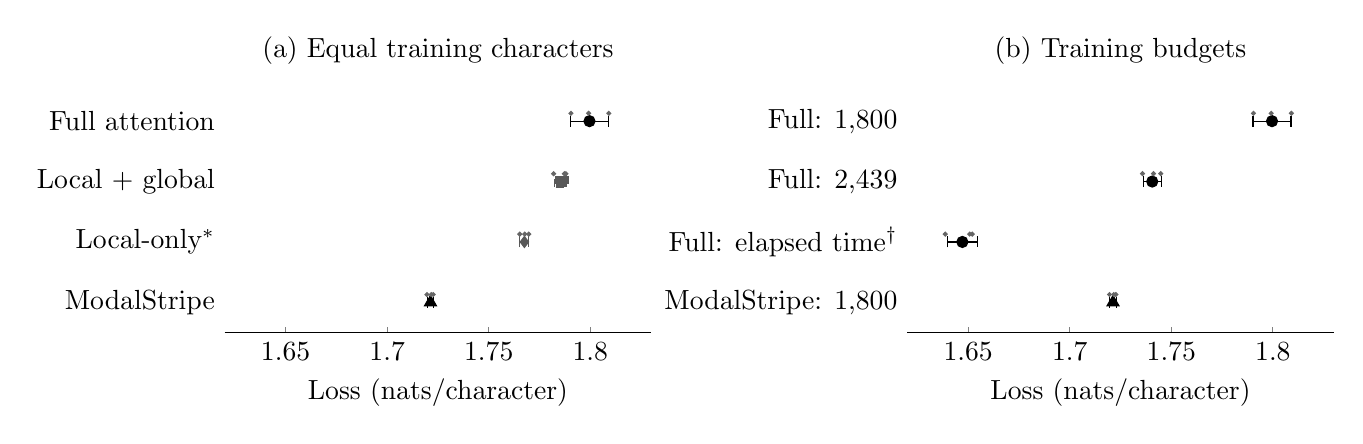
\begin{tikzpicture}
\begin{axis}[name=left,width=7.0cm,height=4.65cm,xmin=1.62,xmax=1.83,ymin=-.5,ymax=3.5,
xtick={1.65,1.70,1.75,1.80},ytick={0,1,2,3},yticklabels={ModalStripe,Local-only$^*$,Local + global,Full attention},xlabel={Loss (nats/character)},title={(a) Equal training characters},ytick style={draw=none},axis y line*=left,y axis line style={draw=none}]
\addplot[black,mark=*,mark options={fill=black},only marks,mark size=2pt,error bars/.cd,x dir=both,x explicit] coordinates {(1.7995751904,3) +- (0.0093327860,0)};
\addplot[only marks,black!60,mark=*,mark size=.7pt] coordinates {(1.8091002695,3.13) (1.7991779166,3.13) (1.7904473851,3.13)};
\addplot[black!65,mark=square*,mark options={fill=black!65},dashed,only marks,mark size=2pt,error bars/.cd,x dir=both,x explicit] coordinates {(1.7856989342,2) +- (0.0033050463,0)};
\addplot[only marks,black!60,mark=*,mark size=.7pt] coordinates {(1.7880092494,2.13) (1.7871743971,2.13) (1.7819131561,2.13)};
\addplot[black!65,mark=diamond*,mark options={fill=black!65},only marks,mark size=2pt,error bars/.cd,x dir=both,x explicit] coordinates {(1.7675650366,1) +- (0.0022196186,0)};
\addplot[only marks,black!60,mark=*,mark size=.7pt] coordinates {(1.7697079469,1.13) (1.7677112260,1.13) (1.7652759369,1.13)};
\addplot[black,mark=triangle*,mark options={fill=black},line width=.9pt,only marks,mark size=2pt,error bars/.cd,x dir=both,x explicit] coordinates {(1.7213171540,0) +- (0.0015783976,0)};
\addplot[only marks,black!60,mark=*,mark size=.7pt] coordinates {(1.7195883558,0.13) (1.7226813346,0.13) (1.7216817716,0.13)};
\end{axis}
\begin{axis}[at={(left.south east)},anchor=south west,xshift=3.25cm,width=7.0cm,height=4.65cm,xmin=1.62,xmax=1.83,ymin=-.5,ymax=3.5,
xtick={1.65,1.70,1.75,1.80},ytick={0,1,2,3},yticklabels={ModalStripe: 1{,}800,Full: elapsed time$^\dagger$,Full: 2{,}439,Full: 1{,}800},xlabel={Loss (nats/character)},title={(b) Training budgets},ytick style={draw=none},axis y line*=left,y axis line style={draw=none}]
\addplot[black,mark=*,mark options={fill=black},only marks,mark size=2pt,error bars/.cd,x dir=both,x explicit] coordinates {(1.7995751904,3) +- (0.0093327860,0)};
\addplot[only marks,black!60,mark=*,mark size=.7pt] coordinates {(1.8091002695,3.13) (1.7991779166,3.13) (1.7904473851,3.13)};
\addplot[black,mark=*,mark options={fill=black},only marks,mark size=2pt,error bars/.cd,x dir=both,x explicit] coordinates {(1.7406215913,2) +- (0.0045175015,0)};
\addplot[only marks,black!60,mark=*,mark size=.7pt] coordinates {(1.7447996544,2.13) (1.7412373075,2.13) (1.7358278118,2.13)};
\addplot[black,mark=*,mark options={fill=black},only marks,mark size=2pt,error bars/.cd,x dir=both,x explicit] coordinates {(1.6471622777,1) +- (0.0073393169,0)};
\addplot[only marks,black!60,mark=*,mark size=.7pt] coordinates {(1.6507480775,1.13) (1.6387194078,1.13) (1.6520193479,1.13)};
\addplot[black,mark=triangle*,mark options={fill=black},line width=.9pt,only marks,mark size=2pt,error bars/.cd,x dir=both,x explicit] coordinates {(1.7213171540,0) +- (0.0015783976,0)};
\addplot[only marks,black!60,mark=*,mark size=.7pt] coordinates {(1.7195883558,0.13) (1.7226813346,0.13) (1.7216817716,0.13)};
\end{axis}\end{tikzpicture}
% END figures/plots/quality.tex
}
\caption{Final-book reset-128 loss for parameter-matched models; lower is better. Large markers are three-seed means, whiskers are sample SDs, and small markers are individual seeds. (a) All models receive 1,800 updates. $^*$Exploratory local-only control. (b) Attention receives different training allowances. $^\dagger$Elapsed-time runs use 4,417, 4,609 and 4,146 updates; changing host load confounds this comparison. Exact scores are in Table~\ref{tab:comparison}.}
\label{fig:quality}
\end{figure}

Under the timing-calibrated allowance, attention improves to PPL 5.701, leaving a hybrid advantage of about 1.9\%. Literal elapsed-time matching instead gives attention 4,417, 4,609 and 4,146 updates and reverses the result. Host-load drift prevents treating that reversal as clean compute matching, but it is important to retain. Neither comparison supports an unconditional training-efficiency claim.

\subsection{CPU latency and cache}
At short prefixes the hybrid is slower than full attention. At 8k, it has faster measured prefill and decoding and roughly half the retained cache (Figure~\ref{fig:resources}). The local-plus-global control saves almost the same cache and runs faster. Removing one global-attention block accounts for most of the storage reduction; the modal state adds only 4\,KiB.

\begin{figure}[htbp]
\centering\resizebox{\textwidth}{!}{
% BEGIN figures/plots/resources.tex
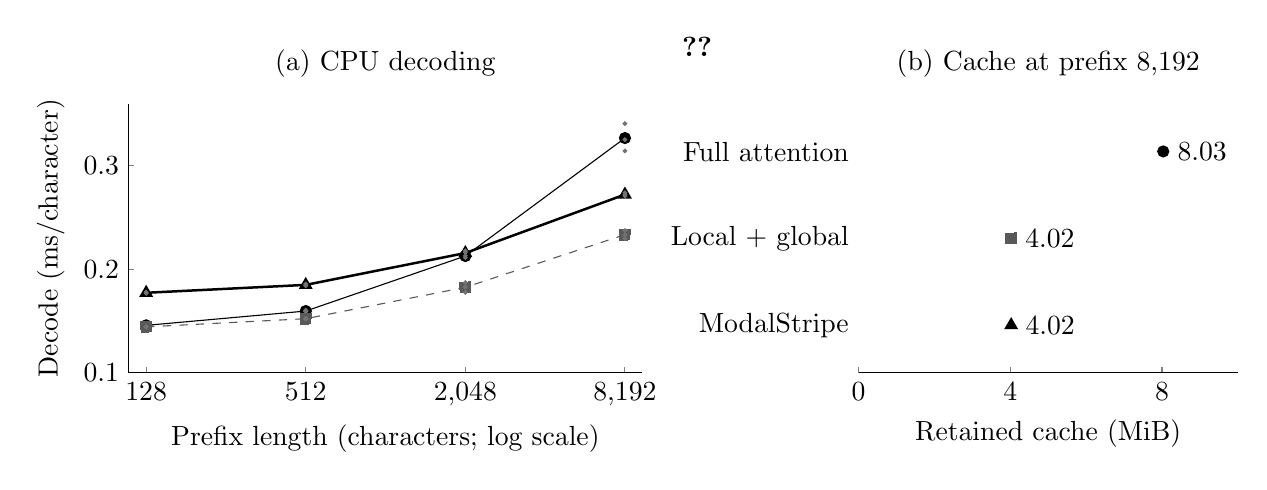
\begin{tikzpicture}
\begin{axis}[name=left,width=8.1cm,height=5.0cm,xmode=log,log basis x=2,xmin=110,xmax=9500,xtick={128,512,2048,8192},xticklabels={128,512,2{,}048,8{,}192},ymin=.1,ymax=.36,ytick={.1,.2,.3},xlabel={Prefix length (characters; log scale)},ylabel={Decode (ms/character)},title={(a) CPU decoding},legend to name=models,legend columns=3]
\addplot[black,mark=*,mark options={fill=black},mark size=2pt] coordinates {(128,0.1458780310) (512,0.1596957500) (2048,0.2128676248) (8192,0.3267986146)};\addlegendentry{Full attention}
\addplot[only marks,black!55,mark=*,mark size=.65pt,forget plot] coordinates {(128,0.1456796872) (128,0.1462031250) (128,0.1457512808) (512,0.1593541874) (512,0.1604713434) (512,0.1592617191) (2048,0.2113189994) (2048,0.2151093749) (2048,0.2121745001) (8192,0.3143554686) (8192,0.3252994684) (8192,0.3407409067)};
\addplot[black!65,mark=square*,mark options={fill=black!65},dashed,mark size=2pt] coordinates {(128,0.1444179688) (512,0.1523029481) (2048,0.1826128434) (8192,0.2335121562)};\addlegendentry{Local + global}
\addplot[only marks,black!55,mark=*,mark size=.65pt,forget plot] coordinates {(128,0.1442656248) (128,0.1444700629) (128,0.1445182188) (512,0.1519453126) (512,0.1525390626) (512,0.1524244690) (2048,0.1777148436) (2048,0.1872513121) (2048,0.1828723744) (8192,0.2374518126) (8192,0.2298971558) (8192,0.2331875003)};
\addplot[black,mark=triangle*,mark options={fill=black},line width=.9pt,mark size=2pt] coordinates {(128,0.1773507086) (512,0.1849761359) (2048,0.2157443541) (8192,0.2722595418)};\addlegendentry{ModalStripe}
\addplot[only marks,black!55,mark=*,mark size=.65pt,forget plot] coordinates {(128,0.1771067809) (128,0.1769036571) (128,0.1780416878) (512,0.1859713757) (512,0.1841445319) (512,0.1848125003) (2048,0.2130703124) (2048,0.2163880317) (2048,0.2177747183) (8192,0.2739453130) (8192,0.2720703123) (8192,0.2707630001)};
\end{axis}
\begin{axis}[at={(left.south east)},anchor=south west,xshift=2.75cm,width=6.4cm,height=5.0cm,xmin=0,xmax=10,xtick={0,4,8},ymin=-.55,ymax=2.55,ytick={0,1,2},yticklabels={ModalStripe,Local + global,Full attention},xlabel={Retained cache (MiB)},title={(b) Cache at prefix 8{,}192},axis y line*=left,y axis line style={draw=none},ytick style={draw=none}]
\addplot[black,mark=*,mark options={fill=black},only marks,mark size=2pt] coordinates {(8.031494141,2)};\node[anchor=west,font=\fontsize{10}{12}\selectfont] at (axis cs:8.151494140625,2){8.03};
\addplot[black!65,mark=square*,mark options={fill=black!65},dashed,only marks,mark size=2pt] coordinates {(4.019775391,1)};\node[anchor=west,font=\fontsize{10}{12}\selectfont] at (axis cs:4.139775390625,1){4.02};
\addplot[black,mark=triangle*,mark options={fill=black},line width=.9pt,only marks,mark size=2pt] coordinates {(4.023681641,0)};\node[anchor=west,font=\fontsize{10}{12}\selectfont] at (axis cs:4.143681640625,0){4.02};
\end{axis}
\node[anchor=south] at ($(left.north east)+(.7,.48)$) {\ref{models}};
\end{tikzpicture}
% END figures/plots/resources.tex
}
\caption{CPU decoding and retained cache for context-128-trained models; lower is better. Apple M1, float32, two threads, batch one, 32-character continuation. (a) Lines join means of three seed medians; small points are seed medians from nine interleaved repeats per seed. The horizontal axis is logarithmic. (b) Retained tensor payload at prefix 8,192, excluding weights and peak process memory. Table~\ref{tab:timing} gives exact values and prefill timing.}
\label{fig:resources}
\end{figure}

At training context 128, mean seed-median step times are 17.289\,ms for attention and 24.411\,ms for the hybrid. The ratio of those means differs from the median paired ratio used for calibration. At context 512 they are 26.445 and 27.903\,ms. These measurements concern this implementation and hardware, not production kernels or GPU throughput.

A later local-only control reaches PPL 5.857. In its separate seed-0 timing audit, it retains only 8.25\,KiB at 8k and decodes faster than the hybrid. It therefore offers a strong resource tradeoff for character prediction. Its bounded receptive field does not provide distant retrieval, however. The architecture control was added after primary outcomes were viewed and remains exploratory; its learning-rate choice still uses development data only.

\subsection{Evaluation beyond the training context}
Our first extrapolation test scored 128 continuation characters after a prefix. Even its 128-prefix condition therefore exceeded the positions seen in context-128 training. We retain it as a continuation test, not a fixed-window baseline. A corrective diagnostic predicts single targets from exactly the named amount of history. It uses seed 0 and 64 fixed positions per book, shared across all input lengths.

\begin{center}\begin{minipage}{\textwidth}\centering\small
\captionof{table}{ModalStripe's corrective fixed-window diagnostic. PPL uses identical target positions at each history length. This small, single-seed audit was added after primary outcomes were inspected. Full comparisons are in Appendix~\ref{app:results}.}
\label{tab:context}

% BEGIN paper/tables/length_summary.tex
\begin{tabular}{rrr}\toprule
Training context & PPL at 128 & PPL at 8,192\\\midrule
128 & 4.599 & 8.781 \\
512 & 5.071 & 6.873 \\
\bottomrule\end{tabular}

% END paper/tables/length_summary.tex

\end{minipage}\end{center}

The drop in quality at longer histories remains clear in this diagnostic. Training at 512 reduces it but does not remove it. Longer history also changes absolute positional indices, so the test cannot separate positional extrapolation from the effects of additional context. Faster processing at 8k should not be read as preserved prediction quality there.

\section{Discussion and conclusion}
The modal branch improves short-window transfer prediction under both allocation rules. Its advantage over attention becomes small under the calibrated training allowance, while simpler attention controls expose useful resource alternatives. These results support a narrow small-model tradeoff.

The evidence covers two final books and three optimization seeds. Training losses are still improving late in the schedule, the selected learning rate is at the grid boundary, and the later context/local-only audits are exploratory. Larger token models, broader tasks, longer training, stronger mixer ablations and optimized GPU comparisons are needed for stronger claims. In particular, the hybrid retains one global-attention block: it has an $O(T)$ KV cache and quadratic attention work, not a bounded-memory or wholly subquadratic architecture.

\paragraph{Acknowledgments.}
OpenAI Codex assisted with implementation, auditing and manuscript preparation.
\label{main:last}
\clearpage

% BEGIN paper/references.tex
\begin{thebibliography}{10}\small\raggedright
\bibitem{vaswani} A. Vaswani et al. \emph{Attention Is All You Need}. 2017. \href{https://arxiv.org/abs/1706.03762}{arXiv:1706.03762}.
\bibitem{fno} Z. Li et al. \emph{Fourier Neural Operator for Parametric Partial Differential Equations}. 2020. \href{https://arxiv.org/abs/2010.08895}{arXiv:2010.08895}.
\bibitem{s4} A. Gu, K. Goel, and C. R\'e. \emph{Efficiently Modeling Long Sequences with Structured State Spaces}. 2021. \href{https://arxiv.org/abs/2111.00396}{arXiv:2111.00396}.
\bibitem{h3} D. Y. Fu, T. Dao, K. K. Saab, A. W. Thomas, A. Rudra, and C. R\'e. \emph{Hungry Hungry Hippos: Towards Language Modeling with State Space Models}. 2022. \href{https://arxiv.org/abs/2212.14052}{arXiv:2212.14052}.
\bibitem{hyena} M. Poli et al. \emph{Hyena Hierarchy: Towards Larger Convolutional Language Models}. 2023. \href{https://arxiv.org/abs/2302.10866}{arXiv:2302.10866}.
\bibitem{stripedhyena} J. Ku et al. \emph{Systems and Algorithms for Convolutional Multi-Hybrid Language Models at Scale}. 2025. \href{https://arxiv.org/abs/2503.01868}{arXiv:2503.01868}.
\bibitem{zoology} S. Arora et al. \emph{Zoology: Measuring and Improving Recall in Efficient Language Models}. 2023. \href{https://arxiv.org/abs/2312.04927}{arXiv:2312.04927}.
\bibitem{ssd} T. Dao and A. Gu. \emph{Transformers are SSMs: Generalized Models and Efficient Algorithms Through Structured State Space Duality}. 2024. \href{https://arxiv.org/abs/2405.21060}{arXiv:2405.21060}.
\bibitem{deltanet} S. Yang, J. Kautz, and A. Hatamizadeh. \emph{Gated Delta Networks: Improving Mamba2 with Delta Rule}. 2024. \href{https://arxiv.org/abs/2412.06464}{arXiv:2412.06464}.
\bibitem{adamw} I. Loshchilov and F. Hutter. \emph{Decoupled Weight Decay Regularization}. 2017. \href{https://arxiv.org/abs/1711.05101}{arXiv:1711.05101}.
\end{thebibliography}
% END paper/references.tex

\clearpage
\appendix
\section{Model and implementation details}\label{app:methods}
The input at position $t$ is $E[x_t]+W_{\mathrm{prev}}E[x_{t-1}]+\operatorname{PE}(t)$, with a zero previous embedding at a window boundary. The sinusoidal encoding uses base 10,000. Each mixer performs a pre-normalized residual update; the mixed block reuses its first normalization parameters before both sequential mixers. A second normalization precedes the feed-forward network, and a final normalization precedes the untied, bias-free output head. Linear maps are bias-free except the affine parameters of layer normalization. The network has no dropout.

In Eq.~\eqref{eq:modal}, $\alpha_r=\exp(\theta_r)$. Initial rates span $1/256$ to $1/2$ logarithmically; frequencies are equally spaced from 0 to $\pi$. Real and imaginary residue components are initialized with standard deviation $0.1/\sqrt8$. Other weights use the archived PyTorch defaults. Pole magnitudes below one do not by themselves bound the gain of the residual model.

For a sequence of length $T$, the kernel includes lags 0 through $T-1$. FFT evaluation pads to the next power of two at least $2T-1$, multiplies input/kernel transforms channelwise, inverts and retains the first $T$ positions. This computes a one-sided convolution. Expanding Eq.~\eqref{eq:state} gives the same operator from zero initial state. Prefill constructs the recurrent state from the observed prefix. States are complex64 and other weights/activations are float32.

Approximate parameter matching chooses each block's feed-forward width as
\[
 d_{\mathrm{ff}}=\max\left(8,\operatorname{round}\frac{50{,}000-P_M-4d}{2d}\right),
\]
where $P_M$ counts mixer parameters and $4d$ counts the two layer normalizations. Full/local blocks use width 261, and the modal/local block 124. In the fixed-width condition, both blocks use 256. Nominal totals include an inherited, inactive 64-parameter frequency-feature vector and, in ModalStripe, one inactive frequency-gate scalar. No frequency features are supplied; these parameters receive no gradients. The paper preserves the archived totals rather than silently changing their definition.

AdamW uses moments $(0.9,0.999)$ and epsilon $10^{-8}$. The primary schedule is cosine with a 0.1 floor. Literal elapsed-time runs decay by elapsed budget; calibrated runs use a fixed 2,439-update schedule. In every condition, matching a seed matches the training-data stream; differently shaped weights need not share an initialization. Training at 512 uses fewer, longer examples at the same character budget and is tuned against reset-128 development loss. No independent convergence or long-window hyperparameter optimum is established.

\subsection{Modal decoding operator and residual blocks}
\begin{figure}[htbp]
\centering\resizebox{\textwidth}{!}{
\begingroup
\tikzset{every node/.style={font=\sffamily\fontsize{9.5}{11.5}\selectfont},
module/.style={draw=black!75,line width=.55pt,fill=white,minimum height=.78cm,align=center,inner xsep=6pt,inner ysep=5pt},
focal/.style={module,fill=tint,draw=accent,line width=.7pt},
flow/.style={-{Latex[length=1.6mm,width=1.1mm]},line width=.6pt,draw=black!85},
label/.style={font=\sffamily\fontsize{9.5}{11.5}\selectfont,align=center},
heading/.style={font=\sffamily\bfseries\fontsize{10}{12}\selectfont,anchor=west},
op/.style={draw=black!80,circle,fill=white,inner sep=0pt,minimum size=4.8mm,font=\normalsize}}
\hyphenpenalty=10000
\exhyphenpenalty=10000

% BEGIN figures/schematics/02-state-cell.tex
\begin{tikzpicture}[x=1cm,y=1cm]
\node[heading] at (0,6.05) {One step of the modal mixer};
\node (a) at (.15,3.05) {$a_t$};
\node[module,text width=1.75cm] (write) at (2.3,3.05) {Write\\$\psi(a_t)$};
\node[module,text width=1.55cm] (broadcast) at (4.7,3.05) {Broadcast\\$\mathcal B$};
\node[op] (add) at (6.7,3.05) {$+$};
\coordinate (tap) at (8.2,3.05);
\node[label,anchor=south] at (8.2,3.4) {$S_t\in\mathbb C^{8\times64}$};
\node[module,text width=1.9cm] (readout) at (11.2,3.05) {Readout\\$\mathcal C(S_t)$};
\node[op] (gate) at (14.0,3.05) {$\odot$};
\node[module,text width=1.15cm] (wo) at (16.0,3.05) {$W_o$};
\node (m) at (18.0,3.05) {$m_t$};
\draw[flow] (a.east)--(write.west);
\draw[flow] (write.east)--node[label,above=3pt] {$u_t$}(broadcast.west);
\draw[flow] (broadcast.east)--(add.west);
\draw[flow] (add.east)--(readout.west);
\fill (tap) circle (1.05pt);
\draw[flow] (readout.east)--node[label,above=3pt] {$z_t$}(gate.west);
\draw[flow] (gate.east)--(wo.west);
\draw[flow] (wo.east)--(m.west);
% Input-dependent read modulation is separate from the state feedback.
\node[module,text width=2.3cm] (read) at (11.2,5.05) {Read gate\\$\rho(a_t)$};
\draw[flow] (.75,3.05)--(.75,5.05)--(read.west);
\fill (.75,3.05) circle (1.05pt);
\draw[flow] (read.east)--(14,5.05)--node[label,right=3pt] {$g_t$}(gate.north);
% The delay is the single persistent modal-state buffer.
\node[focal,text width=2.6cm] (delay) at (8.2,.45) {One-step delay\\$S_{t-1}$};
\node[module,text width=1.7cm] (p) at (4.45,.45) {Transition\\$P S_{t-1}$};
\draw[flow] (tap)--(delay.north);
\draw[flow] (delay.west)--(p.east);
\draw[flow] (p.north)--(4.45,1.85)--(6.7,1.85)--(add.south);
\node[label,anchor=north,text=accent] at (8.2,-.25) {Cached modal state};
\draw[rule,line width=.45pt] (0,-1.05)--(18.3,-1.05);
\node[label,anchor=north west,text width=17.9cm,align=left] at (0,-1.3) {$\mathcal B(u_t)=\mathbf 1_R u_t^{\mathsf T}$ copies each channel into eight modes before addition. $P=\operatorname{diag}(p_1,\ldots,p_8)$ acts on the mode axis. The blue buffer stores 4 KiB per example in complex64; the global attention cache is separate.};
\end{tikzpicture}

\endgroup
% END figures/schematics/02-state-cell.tex
}
\caption{One modal decoding step. The write and read gates depend on normalized input. The fixed broadcast copies each write into all modes before the state addition. The delay is the modal state buffer; the full model also retains a global attention KV cache. Parameters are fixed during decoding.}
\label{fig:statecell}
\end{figure}

For $R=8$ and $d=64$, write the state as $S_t\in\mathbb C^{R\times d}$ and let $P=\operatorname{diag}(p_1,\ldots,p_R)$. Define
\begin{align}
 u_t=\psi(a_t)&=(W_v a_t)\odot\sigma(W_w a_t),&
 g_t=\rho(a_t)&=\sigma(W_r a_t),\\
 \mathcal B(u_t)&=\mathbf 1_R u_t^{\mathsf T},&
 S_t&=P S_{t-1}+\mathcal B(u_t),\quad S_{-1}=0,\\
 z_{t,k}=\mathcal C(S_t)_k&=\operatorname{Re}\sum_{r=1}^{R}c_{r,k}S_{t,r,k},&
 m_t&=W_o(z_t\odot g_t).
\end{align}
Both state summands have shape $R\times d$. Residue multiplication uses no complex conjugation. $P$ is shared across channels; the residues are channel-specific. Gates and projections are nonlinear or linear maps of the current representation as shown; the linear state transition does not make the complete network linear.

Expanding the recurrence gives $S_{t,r,k}=\sum_{j=0}^{t}p_r^{t-j}u_{j,k}$, which recovers Eq.~\eqref{eq:modal}. Prefill constructs $S_{T-1}$ from that weighted sum, separately from the FFT evaluation of sequence outputs. For $N=2^{\lceil\log_2(2T-1)\rceil}$, the latter is
\begin{equation}
 Z=\left[\operatorname{irFFT}_{N}\left(
 \operatorname{rFFT}_{N}(U)\odot\operatorname{rFFT}_{N}(K)\right)\right]_{0:T}.
\end{equation}
The padding and slice compute the causal convolution without circular wraparound.

For the complete first block, the sequential updates are
\begin{align}
 H^m&=H^{(0)}+\operatorname{Modal}(\operatorname{LN}_1(H^{(0)})),\\
 H^a&=H^m+\operatorname{LocalMHA}_{8}(\operatorname{LN}_1(H^m)),\\
 H^{(1)}&=H^a+\operatorname{FFN}_1(\operatorname{LN}_2(H^a)).
\end{align}
The two $\operatorname{LN}_1$ applications share parameters and act on different inputs. The second block is
\begin{align}
 G&=H^{(1)}+\operatorname{GlobalMHA}(\operatorname{LN}_3(H^{(1)})),\\
 H^{(2)}&=G+\operatorname{FFN}_2(\operatorname{LN}_4(G)),
\end{align}
where $\operatorname{FFN}_b(x)=W_{2,b}\operatorname{GELU}(W_{1,b}x)$.

For either attention operator, $q_t^{(h)}=W_Q^{(h)}a_t$, $k_t^{(h)}=W_K^{(h)}a_t$ and $v_t^{(h)}=W_V^{(h)}a_t\in\mathbb R^{16}$. With four heads,
\begin{align}
 A_{t,j}^{(h)}&=\operatorname{softmax}_{j}\left(q_t^{(h)\mathsf T}k_j^{(h)}/\sqrt{16}+M_{t,j}\right),\\
 b_t^{(h)}&=\sum_j A_{t,j}^{(h)}v_j^{(h)},\qquad
 \operatorname{MHA}(a)_t=W_A[b_t^{(1)};\ldots;b_t^{(4)}].
\end{align}
The mask is zero on $0\le j\le t$ for global attention, or $\max(0,t-7)\le j\le t$ for local attention, and $-\infty$ otherwise. Attention selects among stored positions using a query. The modal branch instead reads an accumulated finite state; convolution--recurrence equivalence does not imply equivalence to arbitrary attention.

\section{Data, evaluation and evidence}\label{app:data}
\begin{center}\begin{minipage}{\textwidth}\centering\small
\captionof{table}{Normalized corpus sizes. PG is the Project Gutenberg ebook identifier. Final tests use each complete normalized book. The remaining 10\% of each development-source text is unused in this study.}

% BEGIN paper/tables/datasets.tex
\begin{tabular}{lrrrrr}\toprule
Work & PG & Characters & Train & Develop & Final test\\\midrule
\emph{Hamlet} & 1524 & 178,099 & 142,479 & 17,810 & -- \\
\emph{Alice} & 11 & 144,861 & 115,888 & 14,486 & -- \\
\emph{Moby-Dick} & 2701 & 1,220,651 & 976,520 & 122,065 & -- \\
\emph{Frankenstein} & 84 & 419,429 & -- & -- & 419,429 \\
\emph{Sherlock Holmes} & 1661 & 562,332 & -- & -- & 562,332 \\
\bottomrule\end{tabular}

% END paper/tables/datasets.tex

\end{minipage}\end{center}

The Gutenberg wrappers are removed; selected smart quotes, dashes, ellipses and nonbreaking spaces are mapped to ASCII equivalents, and remaining non-ASCII characters are discarded. The source works had informed the earlier project. The local protocol is not an independent preregistration. Primary model choices were fixed before the final books were fetched; the calibration rule was specified before primary final-score inspection. The local-only control and corrected fixed-window diagnostic are post hoc.

For book $b$ and seed $s$, let $\ell_{b,s}$ be total next-character loss divided by the number of scored targets. Every target is counted once in reset-128 evaluation, so a book of $N$ characters contributes $N-1$ targets. We form $m_s=(\ell_{1,s}+\ell_{2,s})/2$ and report its seed mean and sample SD; reported aggregate PPL is $\exp(\operatorname{mean}_s m_s)$. Seed variability does not quantify uncertainty across books or tasks.

The original continuation audit uses eight blocks/book and scores 128 targets after each prefix. Scored input positions run from prefix$-1$ to prefix$+126$. The corrective audit uses 64 evenly spaced single-target positions/book, beginning no earlier than position 8,192, and exactly 128, 512, 2,048 or 8,192 preceding characters. This distinguishes the input window from a prefix followed by growing continuation history. The diagnostic remains sparse and single-seed, and it does not isolate positional from history-length effects.

Timing uses an Apple M1 with 8 GiB RAM, macOS 15.5, PyTorch 2.15.0, Python 3.13.3 and two threads. Inference records nine randomized/interleaved repetitions per model/seed after warmup, with 32 generated characters. Training timing records 20 repetitions after three warmup updates and excludes data sampling. Raw repetitions are retained. Optimized native full attention and unfused local/modal implementations are not equally engineered backends. The calibration median over 60 paired step-time ratios need not equal a ratio of displayed mean step times.

Pre-training checks cover the sampler's last valid window, target shifts, document boundaries, future influence and gradients, cache growth, local attention against a dense reference, and spectral finite differences. Trained-model checks cover all 36 evaluated checkpoints, including 8k-prefix cache agreement; maximum long-prefix logit discrepancy is $6.2\times10^{-6}$. An exact-block audit found no training substring match among 7,669 nonoverlapping 128-character final-book blocks. It does not guarantee semantic deduplication or general correctness.

Completed runs preserve full configurations, source copies, data hashes, checkpoints and raw measurements. JSON writes are atomic; incomplete runs restart. Run identifiers depend on configuration/code/data/environment records, and checkpoints are hash-verified before reuse. The companion experiment package runs through \texttt{experiments/rigorous/run\_all.py}, archiving old and new evidence around regeneration. The code, saved checkpoints, raw results and manuscript are available at \href{https://github.com/cerebrum101/modal-stripe}{github.com/cerebrum101/modal-stripe}.

The frozen core hashes are:
\begin{center}\small
\begin{tabular}{ll}\toprule File & SHA-256\\\midrule
\texttt{study.py} & \texttt{\scriptsize 77b87f56be8123b8d5e8250428b29b907a127b560bb07aab39f5c6caa1244540}\\
\texttt{model.py} & \texttt{\scriptsize afa4b39a20cac0503caa680ae5edcd56577813ba30794939ec0f5cc51e3b406d}\\\bottomrule
\end{tabular}\end{center}
The source snapshots are Project Gutenberg ebooks \href{https://www.gutenberg.org/ebooks/1524}{1524}, \href{https://www.gutenberg.org/ebooks/11}{11}, \href{https://www.gutenberg.org/ebooks/2701}{2701}, \href{https://www.gutenberg.org/ebooks/84}{84} and \href{https://www.gutenberg.org/ebooks/1661}{1661}. The manuscript evidence manifest identifies the result JSONs and all 36 evaluated run directories.

\section{Additional results}\label{app:results}
\begin{center}\begin{minipage}{\textwidth}\centering\small
\captionof{table}{Final-book reset-128 results. Models use approximately matched parameter counts and context-128 training. Loss is mean $\pm$ sample SD across three seeds. $\dagger$ marks the exploratory local-only control.}
\label{tab:comparison}

% BEGIN paper/tables/comparison.tex
\begin{tabular}{lrrr}\toprule
Model and budget & Updates & Test loss (nats) & PPL\\\midrule
Full attention & 1,800 & 1.7996 $\pm$ 0.0093 & 6.047 \\
Local + global & 1,800 & 1.7857 $\pm$ 0.0033 & 5.964 \\
ModalStripe & 1,800 & 1.7213 $\pm$ 0.0016 & 5.592 \\
Full, calibrated budget & 2,439 & 1.7406 $\pm$ 0.0045 & 5.701 \\
Full, elapsed-time budget & 4,391 avg. & 1.6472 $\pm$ 0.0073 & 5.192 \\
Local-only$^{\dagger}$ & 1,800 & 1.7676 $\pm$ 0.0022 & 5.857 \\
\bottomrule\end{tabular}

% END paper/tables/comparison.tex

\end{minipage}\end{center}

\begin{center}\begin{minipage}{\textwidth}\centering\small
\captionof{table}{CPU inference for context-128-trained models. Prefill includes cache construction. Cache counts retained tensors, including reserved capacity, not weights or peak process memory.}
\label{tab:timing}

% BEGIN paper/tables/timing.tex
\begin{tabular}{rlrrr}\toprule
Prefix & Model & Prefill (ms) & Decode (ms/char) & Cache (KiB)\\\midrule
128 & Full attention & 0.661 & 0.1459 & 160.25 \\
128 & Local + global & 0.742 & 0.1444 & 84.25 \\
128 & ModalStripe & 1.005 & 0.1774 & 88.25 \\
8,192 & Full attention & 201.524 & 0.3268 & 8,224.25 \\
8,192 & Local + global & 115.441 & 0.2335 & 4,116.25 \\
8,192 & ModalStripe & 130.785 & 0.2723 & 4,120.25 \\
\bottomrule\end{tabular}

% END paper/tables/timing.tex

\end{minipage}\end{center}

\begin{center}\begin{minipage}{\textwidth}\centering\small
\captionof{table}{Fixed feed-forward width 256 in each block, context-128 training and 1,800 updates. Unlike parameter matching, this condition permits additional parameters in ModalStripe. Loss is mean $\pm$ sample SD over three seeds.}

% BEGIN paper/tables/fixedff.tex
\begin{tabular}{lrrr}\toprule
Model & Parameters & Loss (nats) & PPL\\\midrule
Full attention & 119,488 & 1.8015 $\pm$ 0.0084 & 6.058 \\
Local + global & 119,488 & 1.7843 $\pm$ 0.0032 & 5.955 \\
ModalStripe & 136,913 & 1.7060 $\pm$ 0.0036 & 5.507 \\
\bottomrule\end{tabular}

% END paper/tables/fixedff.tex

\end{minipage}\end{center}

\begin{center}\begin{minipage}{\textwidth}\centering\small
\captionof{table}{Per-book reset-128 PPL, geometric over three seeds. Calibrated attention uses 2,439 updates; other rows use 1,800. Local-only is exploratory.}

% BEGIN paper/tables/perbook.tex
\begin{tabular}{lrr}\toprule
Model & Frankenstein & Sherlock Holmes\\\midrule
Full attention & 6.081 & 6.014 \\
Local + global & 5.995 & 5.933 \\
ModalStripe & 5.588 & 5.596 \\
Full attention (calibrated) & 5.724 & 5.678 \\
Local-only & 5.874 & 5.839 \\
\bottomrule\end{tabular}

% END paper/tables/perbook.tex

\end{minipage}\end{center}

\begin{center}\begin{minipage}{\textwidth}\centering\small
\captionof{table}{Corrective exact-window diagnostic, seed 0 and the same 64 target characters/book. The input history is exactly the named length. This is a post hoc diagnostic, not a broad long-context benchmark.}

% BEGIN paper/tables/exact.tex
\begin{tabular}{rlrr}\toprule
Train context & Model & PPL, history 128 & PPL, history 8,192\\\midrule
128 & Full attention & 5.734 & 11.048 \\
128 & Local + global & 5.734 & 9.288 \\
128 & ModalStripe & 4.599 & 8.781 \\
512 & Full attention & 6.929 & 9.276 \\
512 & Local + global & 5.292 & 8.983 \\
512 & ModalStripe & 5.071 & 6.873 \\
128 & Local-only & 5.240 & 11.852 \\
\bottomrule\end{tabular}

% END paper/tables/exact.tex

\end{minipage}\end{center}

\begin{figure}[htbp]
\centering\resizebox{\textwidth}{!}{
% BEGIN figures/plots/context.tex
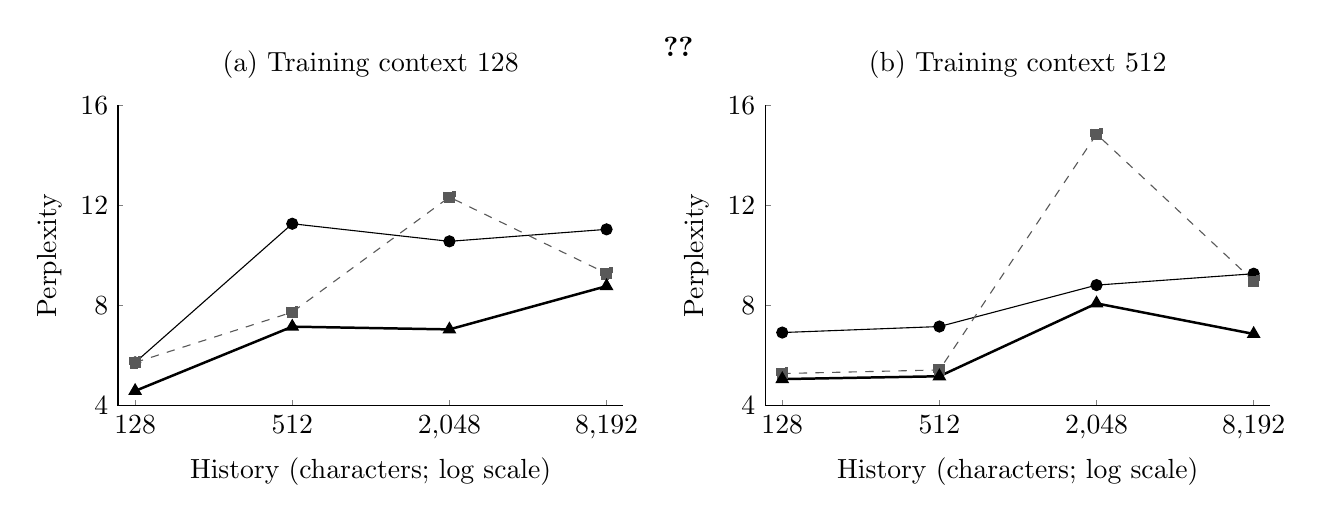
\begin{tikzpicture}\begin{axis}[name=left,legend to name=contextmodels,legend columns=3,width=8cm,height=5.4cm,title={(a) Training context 128},xmode=log,log basis x=2,xmin=110,xmax=9500,xtick={128,512,2048,8192},xticklabels={128,512,2{,}048,8{,}192},ymin=4,ymax=16,ytick={4,8,12,16},xlabel={History (characters; log scale)},ylabel={Perplexity}]
\addplot[black,mark=*,mark options={fill=black},mark size=2pt] coordinates {(128,5.734344991) (512,11.271229965) (2048,10.568611189) (8192,11.047515730)};
\addlegendentry{Full attention}
\addplot[black!65,mark=square*,mark options={fill=black!65},dashed,mark size=2pt] coordinates {(128,5.734232846) (512,7.741930926) (2048,12.335655905) (8192,9.287957445)};
\addlegendentry{Local + global}
\addplot[black,mark=triangle*,mark options={fill=black},line width=.9pt,mark size=2pt] coordinates {(128,4.598926237) (512,7.163514683) (2048,7.054184769) (8192,8.780675376)};
\addlegendentry{ModalStripe}
\end{axis}\begin{axis}[at={(left.south east)},anchor=south west,xshift=1.8cm,width=8cm,height=5.4cm,title={(b) Training context 512},xmode=log,log basis x=2,xmin=110,xmax=9500,xtick={128,512,2048,8192},xticklabels={128,512,2{,}048,8{,}192},ymin=4,ymax=16,ytick={4,8,12,16},xlabel={History (characters; log scale)},ylabel={Perplexity}]
\addplot[black,mark=*,mark options={fill=black},mark size=2pt] coordinates {(128,6.928663367) (512,7.168154634) (2048,8.821584230) (8192,9.276157927)};
\addplot[black!65,mark=square*,mark options={fill=black!65},dashed,mark size=2pt] coordinates {(128,5.292384741) (512,5.436613687) (2048,14.849021225) (8192,8.982725477)};
\addplot[black,mark=triangle*,mark options={fill=black},line width=.9pt,mark size=2pt] coordinates {(128,5.071076171) (512,5.183513027) (2048,8.092098078) (8192,6.872806752)};
\end{axis}\node[anchor=south] at ($(left.north east)+(.7,.5)$) {\ref{contextmodels}};\end{tikzpicture}
% END figures/plots/context.tex
}
\caption{Corrective exact-history diagnostic for all three primary architectures, seed 0, using the same 64 target positions per final book. Lower perplexity is better. Horizontal axes are logarithmic. This exploratory test has no uncertainty estimate; absolute positional indices change with history length.}
\label{fig:contextcurves}
\end{figure}

\begin{center}\begin{minipage}{\textwidth}\centering\small
\captionof{table}{Original prefix-plus-continuation test, three seeds and eight 128-character target blocks/book. Input positions extend beyond the prefix, including in the 128-prefix row.}

% BEGIN paper/tables/continuation.tex
\begin{tabular}{rlrr}\toprule
Train context & Model & PPL, prefix 128 & PPL, prefix 8,192\\\midrule
128 & Full attention & 12.077 & 14.983 \\
128 & Local + global & 8.593 & 11.712 \\
128 & ModalStripe & 7.315 & 9.100 \\
512 & Full attention & 7.216 & 9.844 \\
512 & Local + global & 5.932 & 10.244 \\
512 & ModalStripe & 5.503 & 8.363 \\
\bottomrule\end{tabular}

% END paper/tables/continuation.tex

\end{minipage}\end{center}

\begin{center}\begin{minipage}{\textwidth}\centering\small
\captionof{table}{Context-512-trained models tested with reset-128 windows on the complete final books. This evaluation context differs from training.}

% BEGIN paper/tables/longtrain.tex
\begin{tabular}{lrr}\toprule
Model & Loss (nats) & PPL\\\midrule
Full attention & 2.0051 $\pm$ 0.0060 & 7.427 \\
Local + global & 1.8211 $\pm$ 0.0115 & 6.179 \\
ModalStripe & 1.7508 $\pm$ 0.0028 & 5.759 \\
\bottomrule\end{tabular}

% END paper/tables/longtrain.tex

\end{minipage}\end{center}

\begin{center}\begin{minipage}{\textwidth}\centering\small
\captionof{table}{Development learning curves for approximately matched parameters and context-128 training. Values average three seeds and three source works. All checkpoints share the 1,800-update schedule; continued late improvement is not convergence.}

% BEGIN paper/tables/learning.tex
\begin{tabular}{lrr}\toprule
Model & Update & Development loss (nats)\\\midrule
Full attention & 300 & 2.1684 \\
Full attention & 600 & 2.0316 \\
Full attention & 1200 & 1.8878 \\
Full attention & 1800 & 1.8387 \\
Local + global & 300 & 2.0946 \\
Local + global & 600 & 1.9669 \\
Local + global & 1200 & 1.8575 \\
Local + global & 1800 & 1.8201 \\
ModalStripe & 300 & 2.0451 \\
ModalStripe & 600 & 1.9053 \\
ModalStripe & 1200 & 1.7942 \\
ModalStripe & 1800 & 1.7588 \\
\bottomrule\end{tabular}

% END paper/tables/learning.tex

\end{minipage}\end{center}

\begin{center}\begin{minipage}{\textwidth}\centering\small
\captionof{table}{Interleaved training-step timing: three warmup updates, then 20 repetitions per seed. Batch size is 16 at 128 and 4 at 512. Means of per-seed medians include forward, loss, backward, clipping and AdamW, but exclude data sampling.}

% BEGIN paper/tables/train_timing.tex
\begin{tabular}{rlr}\toprule
Context & Model & Step (ms)\\\midrule
128 & Full attention & 17.289 \\
128 & Local + global & 19.812 \\
128 & ModalStripe & 24.411 \\
512 & Full attention & 26.445 \\
512 & Local + global & 23.439 \\
512 & ModalStripe & 27.903 \\
\bottomrule\end{tabular}

% END paper/tables/train_timing.tex

\end{minipage}\end{center}

\begin{center}\begin{minipage}{\textwidth}\centering\small
\captionof{table}{Separate exploratory local-only timing at prefix 8,192, seed 0, nine randomized paired repeats. These measurements were collected separately from Table~\ref{tab:timing}.}

% BEGIN paper/tables/localtiming.tex
\begin{tabular}{lrr}\toprule
Model & Decode (ms/char) & Cache (KiB)\\\midrule
Full attention & 0.3716 & 8,224.25 \\
ModalStripe & 0.3224 & 4,120.25 \\
Local-only & 0.1979 & 8.25 \\
\bottomrule\end{tabular}

% END paper/tables/localtiming.tex

\end{minipage}\end{center}

For batch one, two full-attention blocks retain $16d(T+32)+4d$ bytes of tensor payload under the allocation policy. ModalStripe retains
\[
 8d(T+32)+8wd+8Rd+4d,
\]
corresponding to one global KV cache, local KV state, complex modal state and the previous embedding. At $d=64,w=8,R=8$, the modal state is 4 KiB. Local plus global removes that state; two local blocks retain $16wd+4d=8,448$ bytes. These formulas exclude weights, workspaces, allocator overhead and process memory. The local-only model's bounded receptive field does not establish distant recall; the project's earlier recall runs trained separate models and are not evidence of retrieval ability in these text-trained checkpoints.
\end{document}
